Экспериментальная апробация разработанных алгоритмов производилась на лабораторном источнике
рентгеновского излучения - трехкристальном рентгеновском спектрометр (ТРС) (рис. \ref{ris:trs}).
ТРС включает в себя рентгеновский источник, спектр является характеристическим и
определяется материалом анода, в частном случае молибденом. Рентгеновские
лучи от неподвижного источника, падают на кристалл-монохроматор, где происходит
пространственное разделение спектра и монохроматизация пучка. Коллимационная щель №1
вырезает необходимую составляющую, которая затем отражается от исследуемого кристалла-образца.

\begin{figure}[H]
  \centering
  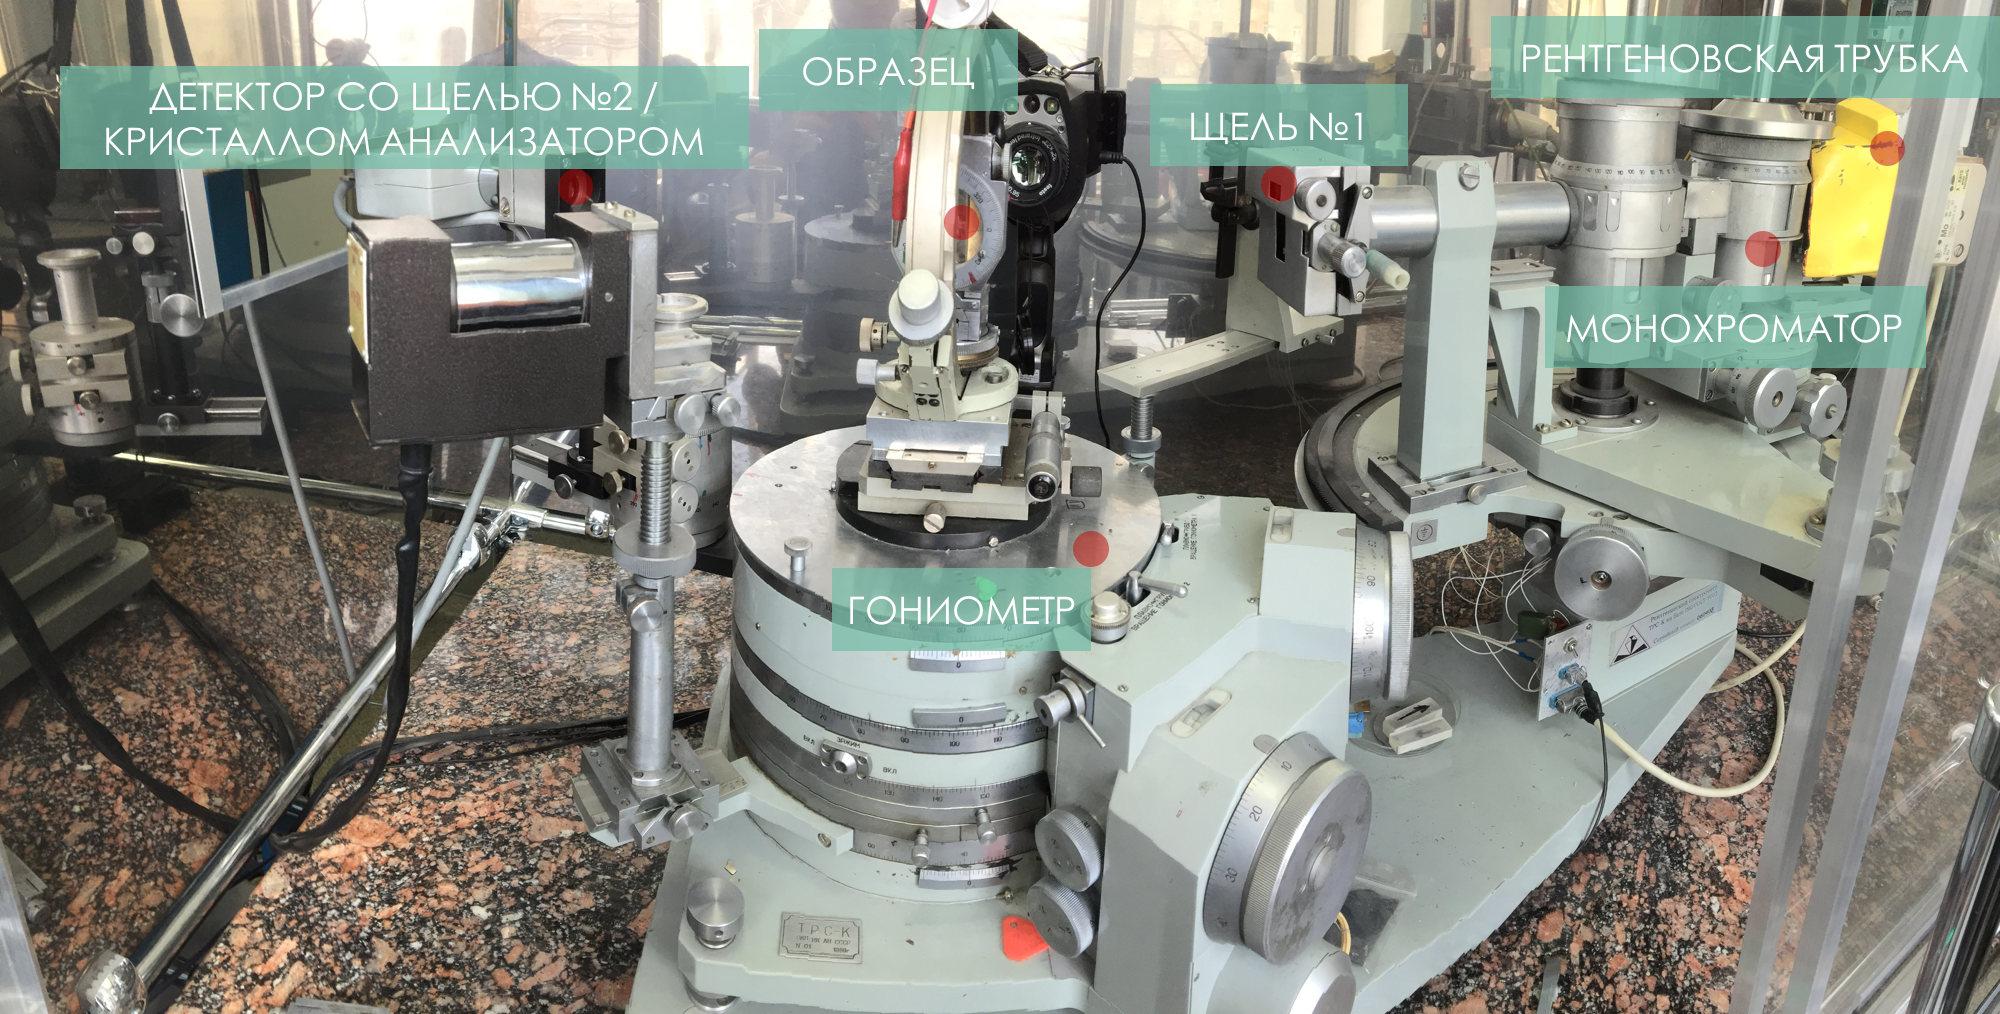
\includegraphics[width=1\textwidth]{images/trs.png}
  \caption{ Трехкристальный рентгеновский спектрометр. Лаборатория рентгеновских
  методов анализа и синхратронного излучения, ФНИЦ "Кристаллография и фотоника"}
  \label{ris:trs}
\end{figure}

Конструкция ТРС предусматривает возможность работать как в режиме двухкристального эксперимента,
когда перед детектором устанавливается коллимационная щель №2,
так и в режиме трехкристального эксперимента, когда на место
 перед детектором устанавливается кристалл анализатор и отраженный от анализатора луч
фиксируется детектором.

Оптическое расстояние от источника до коллимационной щели №1 и №2 составляет 570 мм
и 1005 мм соответсвенно. Кристалл-образец устанавливается на многокружный гониометра с радиусом
(расстоянием до детектора) равным 210 мм, позволяющим осуществлять позиционирование образца и детекторов
 с точностью 0.5 угл. сек. Также ТРС оснащен двумя сцинтилляционнымы детекторами для
проведения методами многоволновой и квазимноговолновой дифракции.
